\documentclass[9pt]{beamer-control}
\usepackage{beamer-control-prac}
\begin{document}
\TOPIC[3]{Frequency Domain}
\CONCEPT[6]{Week 6: Frequency domain analysis}

\begin{frame}
\frametitle{Introduction}
In this practical, we will perform frequency domain analysis of the compound pendulum system using Bode and Nyquist plots.

\vfill

This practical will consist of the following parts:
\begin{itemize}
\item Theoretical analysis
\item Experimental analysis
\end{itemize}
\end{frame}


\SUBCONCEPT{Theoeretical analysis}

\begin{frame}{Compound pendulum}
The theoretical model for the compound pendulum system is given by the transfer function
\[\frac{\theta_m(s)}{v_m(s)} = \frac{114.1}{s^2 + 5.248s+235.1}. \]
Suppose someone implements a poor low-pass filter in the electronics/hardware, say a low pass filter with a cutoff frequency of 10 rad/s. The transfer function with this filter is then
\[\frac{\theta_m(s)}{v_m(s)} = \frac{114.1}{s^2 + 5.248s+235.1}\frac{10}{s+10}. \]
In this practical you will need to use the \textbf{modified} QUBE block, which includes this problematic filter.
\end{frame}

\begin{frame}{Frequency analysis}
Based on this model of the compound pendulum, use Matlab to plot the Bode and Nyquist curves. You will need to enter the transfer function with the low-pass filter as the transfer function myTF.

\includematlab{prac6.m}{part1} 

Inspect the plots to identify regions of interest and consider which range of frequencies should be sampled.

\end{frame}

\SUBCONCEPT{Experimental analysis}

\begin{frame}{Frequency analysis}
The Bode and Nyquist curves can all be constructed from knowledge of the phase and amplitude of the output signal of a plant driven at a range of input frequencies. 

\begin{itemize}
	\item The code on the following slides will produce points on the diagrams to compare these experimental results with the previously plotted theoretical plots
	\item You will need to provide the name of your Simulink model, a range of frequencies (around 10 different frequencies in rad/s) to run the system at, and the name of your input and output signals as given by the To Workspace blocks in Simulink
	\item Using knowledge of how the Bode and Nyquist plots are constructed (such as in the lecture notes), fill in the places in the code surrounded by <> to populate your experimental points on the curves
\end{itemize}
 
\end{frame}

\begin{frame}{Frequency analysis}
	\includematlab{prac6.m}{part2} 
\end{frame}

\begin{frame}{Frequency analysis}
\includematlab{prac6.m}{part3} 
\end{frame}

\begin{frame}{Experimental plots}
You should receive something that looks similar to the below plots.
\begin{figure}
	\centering
	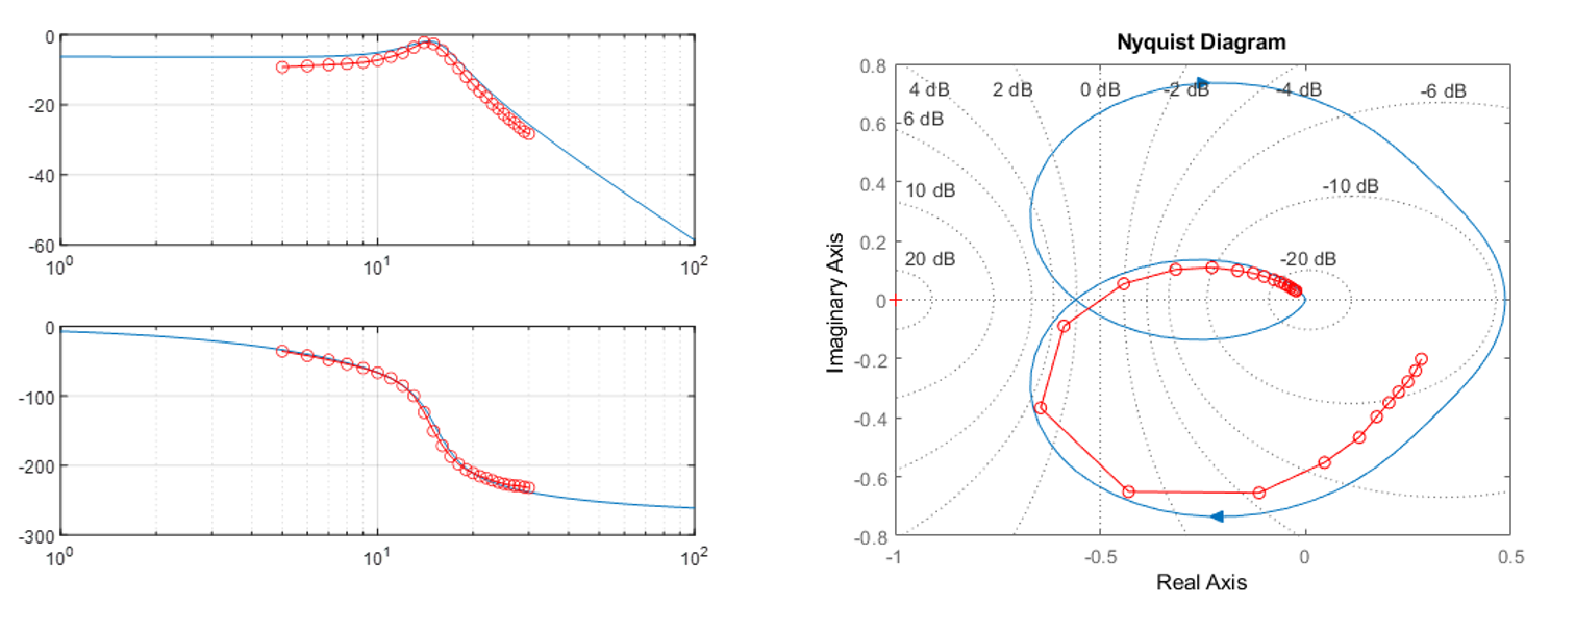
\includegraphics[width=\linewidth]{prac6_experimental}
\end{figure}
\end{frame}


\begin{frame}{System characteristics}
These plots provide us with a wealth of information of our system such as 
\begin{itemize}
	\item Resonant frequency
	\item Stability 
	\item Gain and phase margins
\end{itemize}
Determine these properites of the system by reading their definitions in the lecture notes
\end{frame}


\begin{frame}{Next week}
	This week you theoretically and experimentally analysed the frequency response of the compound pendulum system using Bode and Nyquist plots. 
	
	This concludes the standard practical topics using the QUBEs and next week we will begin the practical project using the ping pong rig.
\end{frame}



\end{document}
